\section{Auswertung}
\label{sec:Auswertung}


\subsection{Biometrische Untersuchung eines Augenmodells}

In Abbildung \ref{fig:Auge} ist der A-Scan des Augenmodells aufgeführt.
\begin{figure}
  \centering
  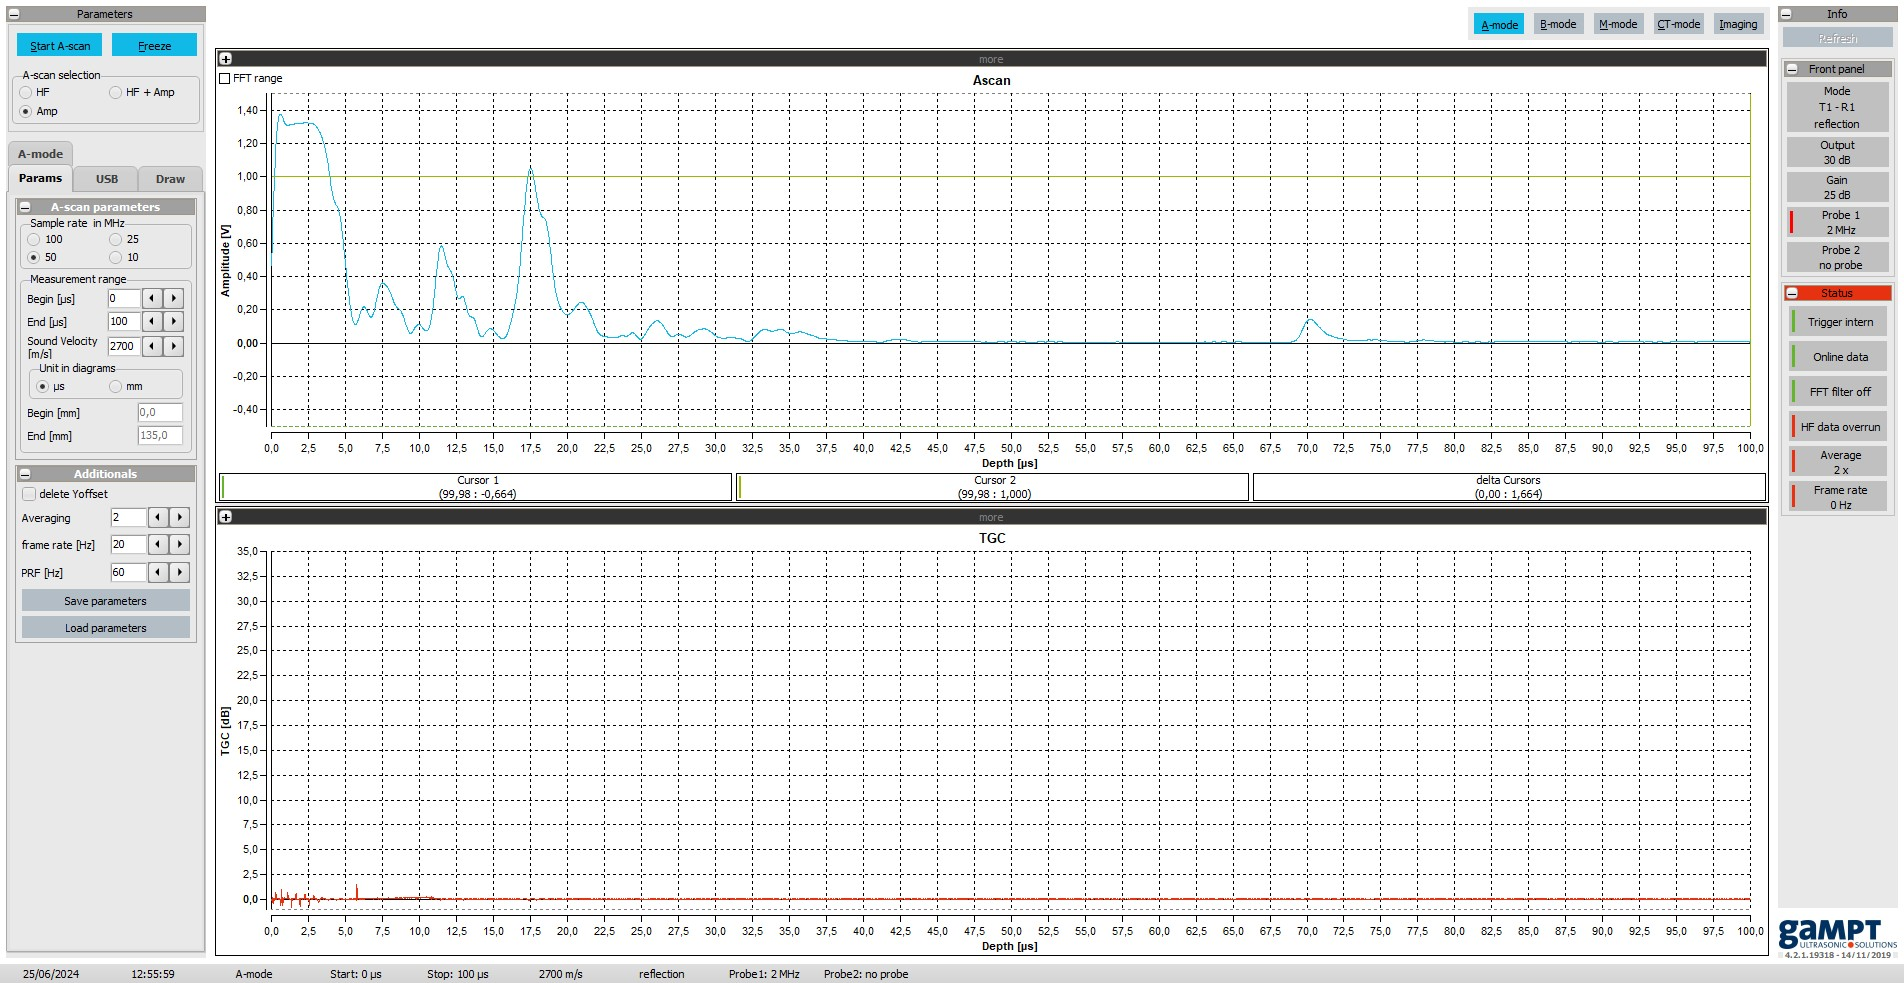
\includegraphics[width=\textwidth]{Bilder/Auge1.jpg}
  \caption{Abgebildet ist die Vermessung des Augenmodells mit dem A-Scan Verfahren}
  \label{fig:Auge}
\end{figure}

Die Zeiten, bei denen die Peaks auftreten, sind
\begin{gather*}
  t_{Iris}=   \qty{7.57}{\micro\second}
  t_{Linse_1}=\qty{11.56}{\micro\second}
  t_{Linse_2}=\qty{17.51}{\micro\second}
  t_{Retina}= \qty{70.17}{\micro\second} \qquad .
\end{gather*}

\noindent Zur Berechnung der Strecken wird von jedem dieser Werte $\frac{x_M}{c_A}$ abgezogen.
Mit der Schallgeschwindigkeit für die Glaskörperflüssigkeit $c_{GK}=\qty{1410}{\meter\per\second}$ lässt sich beim multiplizieren mit $t_{Iris}$ die Strecke bis zur Iris bestimmen.
Genau dasselbe wird für die Strecke zur Linse mit $t_{Linse_1}$ gemacht.
Danach muss für die Strecke in der Linse die Schallgeschwindigkeit $c_L=\qty{2500}{\meter\per\second}$ benutzt werden.
Bei dem Stück von dem Ende der Linse bis zur Retina wird wieder die Schallgeschwindigkeit der Glaskörperflüssigkeit verwendet.
Damit erbgeben sich die Werte
\begin{gather*}
  s_{Iris}=     \qty{8.1(0.6)}{\micro\second}
  s_{Linse_1}= \qty{13.7(0.6)}{\micro\second}
  s_{Linse_2}= \qty{28.6(0.6)}{\micro\second}
  s_{Retina}= \qty{102.9(0.6)}{\micro\second} \qquad .
\end{gather*}


\subsection{Untersuchung eines Brustmodells mit einem B-Scan}

In Abbildung \ref{fig:Brust} wird der B-Scan des Brustmodells dargestellt.
Durch grafische Auswertung wird dann die Breite von dem linken Tumor, mit $b_1=\qty{17.27}{\milli\meter}$ und die des rechten, mit $b_2=\qty{15.95}{\milli\meter}$, bestimmt.
Mit der Annahme, die Tumore seien Kugeln, wird deren Volumen ausgerechnet.
Es ergibt sich $V_1=\qty{234.25}{\milli\meter\cubed}$ und $V_2=\qty{199.81}{\milli\meter\cubed}$.
Zudem wird grafisch die Tiefe der Tumore, mit $d_1=\qty{17.11}{\milli\meter}$ und $d_2=\qty{11.39}{\milli\meter}$, gemessen.
Da Tumor 2 auf dem Bild vergleichsweise sehr hell erschein, handelt es sich bei diesem wahrscheinlich um einen, aus festem Gewebe bestehenden Tumor.
Bei Tumor 1 ist zu vermuten, dass es sich bei diesem um einen mit Flüssigkeit gefüllten Tumor, also um eine Zyste, handelt, da dieser weniger hell ist. 

\begin{figure}
  \centering
  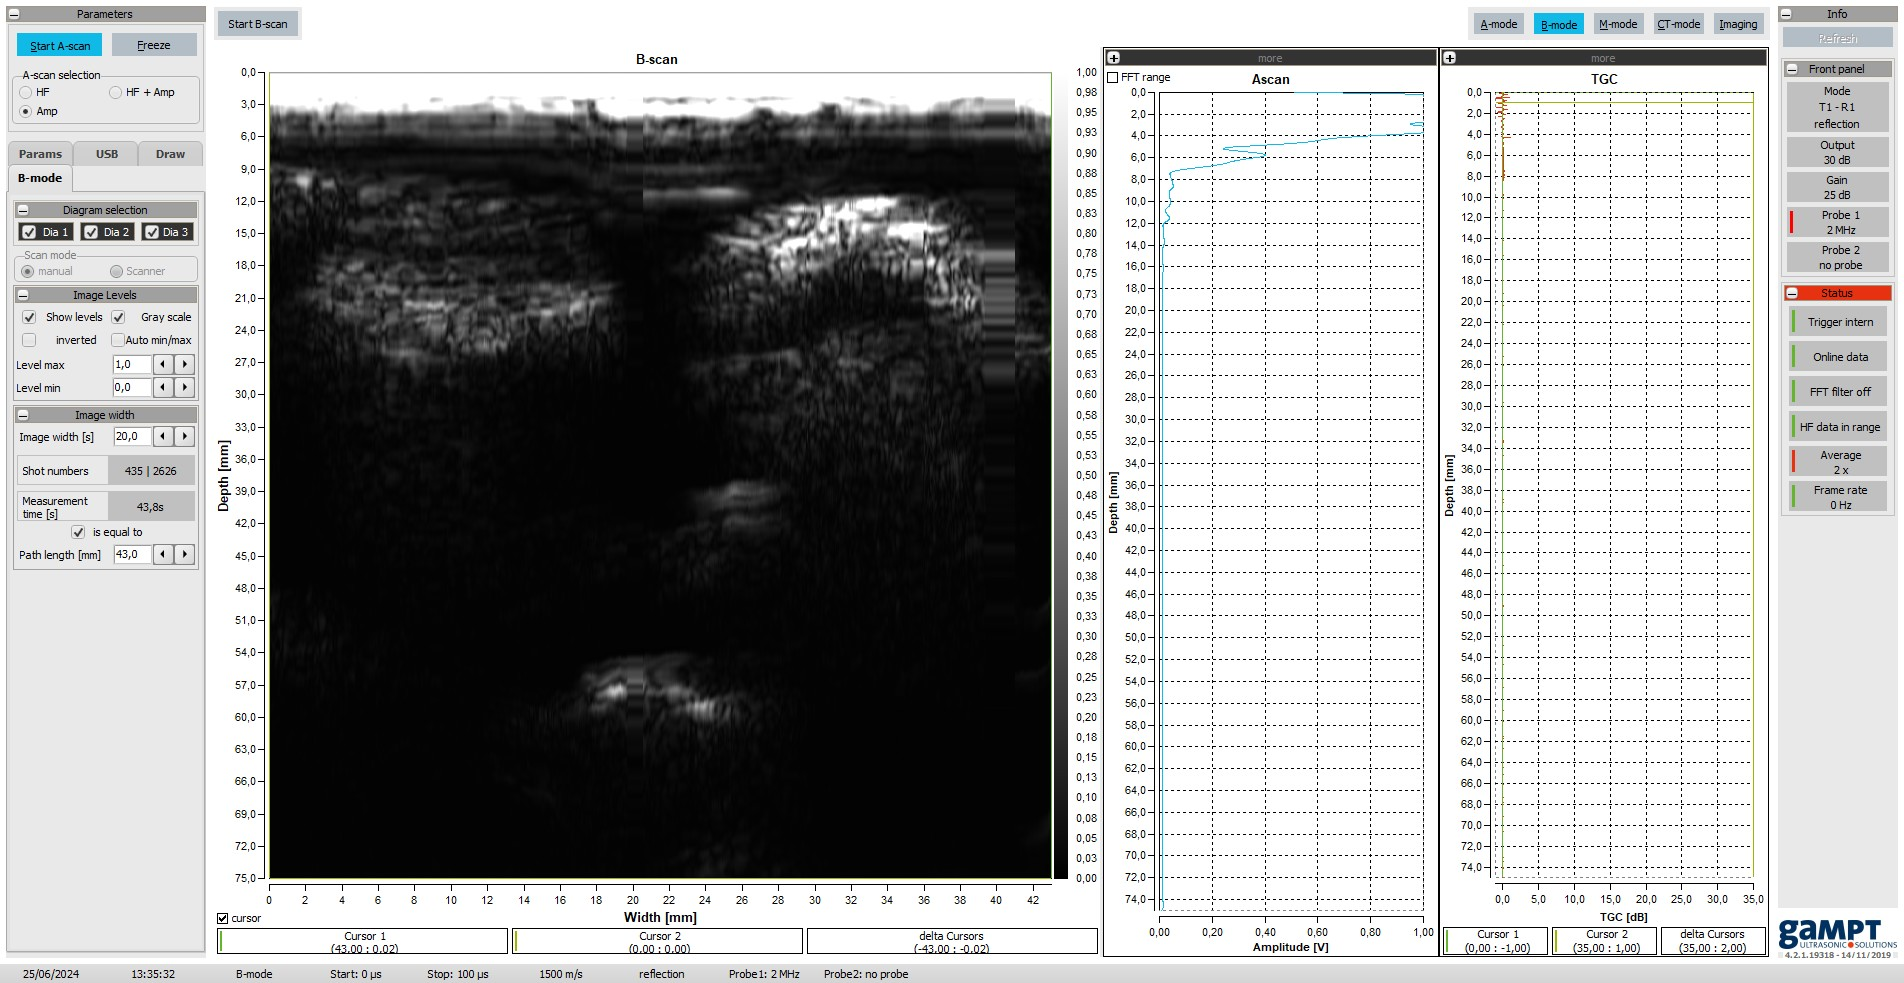
\includegraphics[width=\textwidth]{Bilder/Brust6.jpg}
  \caption{hHier ist Untersuchung des Brustmodells mithilfe des B-Scan Verfahrens aufgezeigt.}
  \label{fig:Brust}
\end{figure}

\subsection{Untersuchung eines Herzmodells mit einem TM-Scan}

Für die Untersuchung des Herzmodells wurden die Werte in Tabelle \ref{tab:Herz} aufgenommen.
$d$ ist dabei die gemessene Tiefe der Maxima unter dem Nullpunkt. 
Die Höhe der Peaks kann dann mit $h=\qty{75}{\milli\meter}-d-h_0$ bestimmt werden, wobei $h_0=44.21$ der gemessenen Baseline entspricht.

\begin{table}[H]
  \centering
  \caption{Höhe und Breite der Peaks beim TM-Scan des Herzmodells.}
  \label{tab:Herz}
  \sisetup{table-format=1.1, per-mode=reciprocal}
  \begin{tblr}{
      colspec = {S[table-format=3.0] S[table-format=2.1] S},
      row{1} = {guard, mode=math},
    }
    \toprule
    d \mathbin{/} \unit{\milli\meter} & \increment t \mathbin{/} \unit{\second}  \\
    \midrule
    17.85 &  1.33\\
    21.03 &  1.12\\
    21.75 &  1.02\\
    24.03 &  1.03\\
    24.12 &  1.97\\
    24.57 &  0.87\\
    26.11 &  0.93\\
    26.66 &  0.95\\
    25.93 &  0.95\\
    25.75 &  0.86\\
    \bottomrule
  \end{tblr}
\end{table}



